\documentclass[10pt,conference,letterpaper]{IEEEtran}
\usepackage{amsmath,amssymb}
\usepackage{graphicx}
\usepackage{booktabs}
\usepackage{microtype}
\usepackage{url}
\graphicspath{{figures/}}
\setlength{\textfloatsep}{6pt plus 1pt minus 2pt}
\setlength{\floatsep}{6pt plus 1pt minus 2pt}

\title{Reproducible Target-Informed Gaussian-Process Optimization for Data-Efficient Electromagnetic Design}
\author{\IEEEauthorblockN{Le Dong}
\IEEEauthorblockA{\textit{School of Electrical Engineering}\\
\textit{Xi'an Jiaotong University}\\
Xi'an, Shaanxi 710049, China\\
\texttt{leroi\_2024@stu.xjtu.edu.cn}}}

\begin{document}
\maketitle

\begin{abstract}
Electromagnetic design often requires a prescribed response band while minimizing a second response under a small observation budget. We construct a reproducible target-informed Gaussian-process (GP) workflow, rather than a new acquisition: deterministic center initialization, uncertainty-aware feasibility discovery, fixed GP starts, a dimension-aware evidence guard, relative constrained-expected-improvement (cEI) stopping, and charged confirmation. Frozen after 14 development targets, it recovers every exhaustive optimum at the other 73 targets of a 1,110-design coil lattice with 21.81 mean calls. Random-six initialization with the same stopping machinery recovers 856/870 seed--target optima and remains seed-dependent, whereas center-start trajectories are invariant. On a 21-target, eight-dimensional wireless-power-transfer (WPT) benchmark, the workflow and matched conventional cEI satisfy 21/21 targets, versus 10/21 for Sobol search; stopping saves 30.3\% of calls with a 3.79\% resistance penalty. In a separate matched 1000-nH Maxwell execution, both policies use 30 accepted evaluations and qualify, while the automatic workflow returns $0.38368~\Omega$ versus $0.38954~\Omega$. The contribution is reproducible observation-budget allocation, not universal optimizer superiority.
\end{abstract}

\begin{IEEEkeywords}
Bayesian optimization, constrained expected improvement, electromagnetic design, Gaussian process, wireless power transfer.
\end{IEEEkeywords}

\section{Introduction}
Electromagnetic design frequently asks for a configuration whose compulsory response lies in a narrow band while another response is optimized. If an expensive oracle returns constrained response $g(x)$ and scalar objective $J(x)$, the task is
\begin{equation}
 \min_{x\in\mathcal X}J(x)\quad\mathrm{s.t.}\quad
 |g(x)-g_t|/|g_t|\leq\epsilon .
 \label{eq:problem}
\end{equation}
The objective can be resistance or a scalarized combination of loss, mass, temperature, material use, and efficiency. A low evaluation count is valuable when each observation requires simulation or measurement, but it also makes initialization, stochastic GP fitting, and stopping materially affect the returned design.

Gaussian-process Bayesian optimization (BO) is established in electromagnetic design. Online GP-assisted evolutionary search has been applied to antennas \cite{liu2014}, machine-learning-assisted antenna optimization has combined learned representations and GPs \cite{wu2024}, and BO has been used for WPT coil design \cite{sim2023}. Constrained expected improvement (cEI) is likewise established \cite{gardner}. Existing studies commonly report performance under fixed budgets, whereas initialization, GP-fit reproducibility, adaptive stopping, and separately charged terminal confirmation are less often evaluated within one auditable observation ledger. We address this workflow-level gap: how should a target-conditioned optimizer spend and stop a small, explicitly counted observation budget reproducibly?

This question connects three issues that are often reported separately. Initial-design size and placement can materially affect small-budget BO \cite{furuuchi2024}; random restarts in GP hyperparameter fitting can make identical data yield different numerical trajectories; and a fixed budget gives no task-dependent indication of when another expensive observation has little posterior value. Formal BO stopping criteria have been derived from posterior simple-regret reduction \cite{ishibashi2023}. We instead study a simpler engineering threshold and test it against exhaustive optima. Its empirical status is explicit: it is a frozen rule supported on the stated domains, not a general convergence theorem.

We make three contributions: matched screens select active GP sampling and cEI; an auditable workflow combines deterministic feasibility discovery and fitting with $B=N_0+N_{\rm seq}+N_{\rm conf}$ accounting and guarded stopping; and frozen settings are tested on 73 held-out exhaustive targets, 21 numerical WPT targets, and a matched-budget direct Maxwell case. The claim concerns reproducibility and budget control, not invention of cEI or universal advantage over conventional BO.

\section{Models and Optimization Method}
\subsection{Two-Dimensional Coil Oracle}
The first controlled oracle describes a multilayer air-core coil by radial layers $T\in\{1,\ldots,10\}$ and turns per layer $n\in\{20,\ldots,130\}$. With wire diameter $d=0.68$ mm, pitch $p=1.05d$, inner diameter $D_0=80$ mm, mean diameter $D=D_0+Tp$, height $H=np$, radial thickness $C=Tp$, total turns $N=Tn$, and resistivity $\rho=1.851\times10^{-5}\ \Omega\,\mathrm{mm}$, the oracle is
\begin{equation}
 L=\frac{0.08N^2D^2\,10^{-4}}{3D+9H+10C}\ {\rm mH},\qquad
 R=\frac{4\rho ND}{d^2}.
 \label{eq:coil}
\end{equation}
The domain contains 1,110 integer designs. A design is feasible when $|L-L_t|/L_t\leq0.025$, and the objective is the smallest feasible $R$. Enumeration supplies an independent reference optimum for each target $L_t=1,\ldots,87$ mH. For a feasible returned design, bounded loss is $u=r/(1+r)$, where $r=R/R_{\rm exhaustive}-1$; infeasible returns have $u=1$.

\subsection{Reusable-Surrogate Screening}
Before target-specific optimization, we compare reusable dual-response GPs and ten-member neural ensembles under the same $B=15+12=27$ protocol: 15 globally reusable model-building observations and 12 target-specific validations. The random policies use 15 seeded uniform observations. Active policies begin with six of the same observations and acquire nine more using equally weighted, scale-normalized uncertainty in $L$ and $R$. Every model family then uses the same validation score and decision pool.

Fig.~\ref{fig:surrogates} shows that active selection helps both families, but the GP is markedly more data-efficient. Random GP sampling qualifies 99.66\% of 870 cases and reaches 658 exact optima; active GP sampling qualifies every case, reaches 759 exact optima, and reduces all-case mean bounded loss from 0.0111 to 0.00218, an 80.3\% reduction. For the tested 16--8 ReLU ensemble, active sampling raises exact recovery from 351 to 586 but leaves mean loss at 0.188. These results select the GP for the target-conditioned study; they do not establish inferiority of neural surrogates generally.

\begin{figure}[!t]
 \centering
 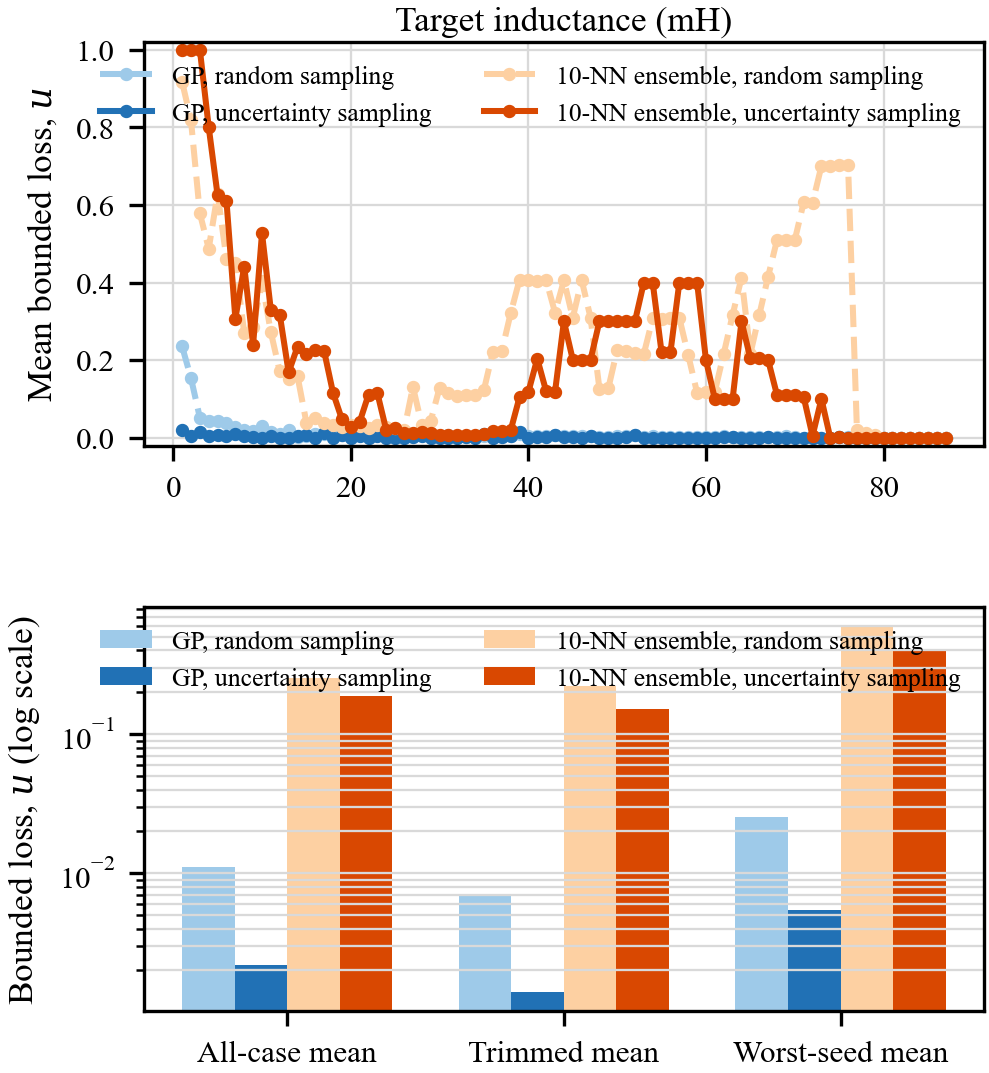
\includegraphics[width=0.90\columnwidth]{fig01_global_surrogate_2x2.png}
 \caption{Matched reusable-surrogate screen at nominal per-target $B=27$. Both model families use 15 shared model-building observations and the same 12 target-specific validations. Lower bounded loss is better.}
 \label{fig:surrogates}
\end{figure}

\subsection{Direct-Search Reference}
We also compare the selected reusable GP with simulated annealing (SA), which searches the integer domain directly using cached evaluations and stops after five cycles without a 1\% feasible-objective improvement \cite{kirkpatrick}. Both methods use the same $\pm2.5\%$ feasibility rule and the same ten seeds. Fig.~\ref{fig:gp-sa} shows trimmed mean bounded loss of 0.00139 for the GP and 0.0451 for SA, at 27 nominal calls versus 92.1. Moreover, the GP's 15 model-building observations are reused across all targets, whereas SA starts a separate search for every target. This benchmark-specific result justifies developing the GP route; it is not a claim that BO generally dominates direct optimization.

\begin{figure}[!t]
 \centering
 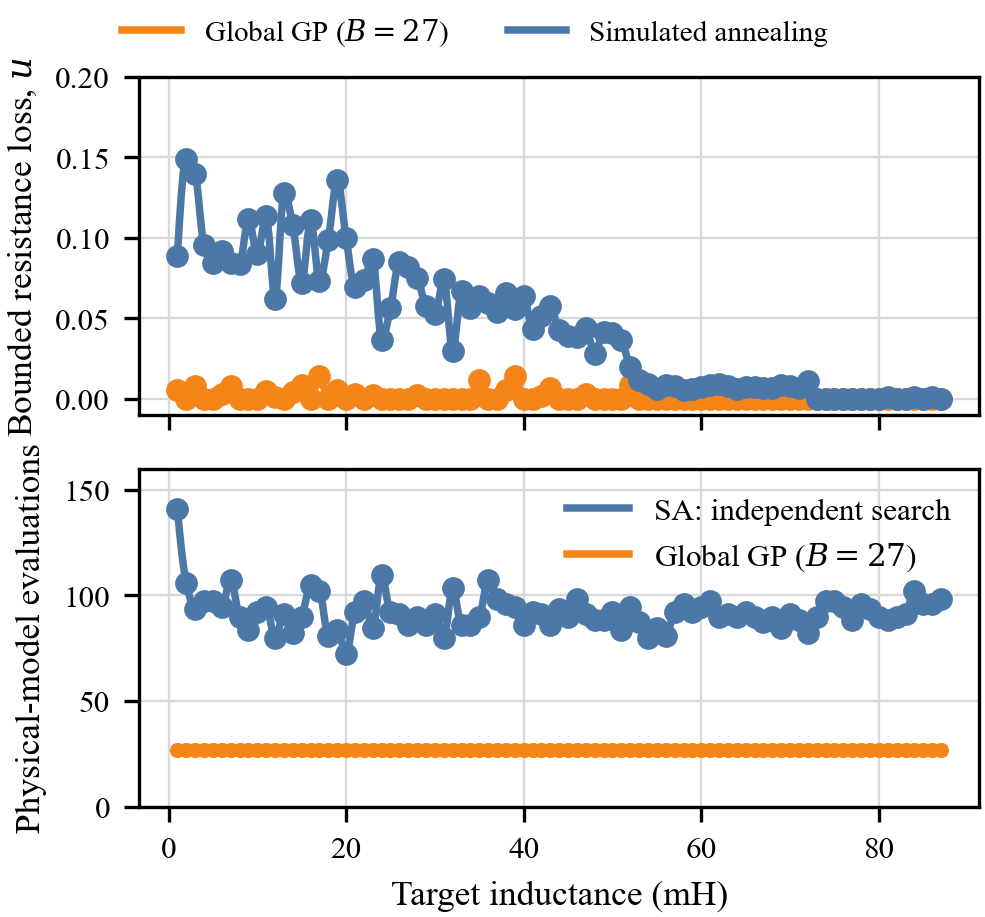
\includegraphics[width=0.90\columnwidth]{fig03_gaussian_process_vs_sa.png}
 \caption{Reusable active GP versus direct SA. The upper panel reports targetwise-trimmed bounded loss and the lower panel physical-model calls. Lines only aid reading between integer targets.}
 \label{fig:gp-sa}
\end{figure}

\subsection{Target-Conditioned Acquisition}
Independent GPs model $L$ and $R$ with radial-basis-function kernels and white-noise terms \cite{rasmussen}. For target $L_t$, the inductance GP gives
\begin{equation}
 p_F(x)=\Phi\!\left(\frac{L_t(1+\epsilon)-\mu_L}{\sigma_L}\right)
 -\Phi\!\left(\frac{L_t(1-\epsilon)-\mu_L}{\sigma_L}\right).
 \label{eq:pf}
\end{equation}
After a feasible observation exists, cEI maximizes $a_{\rm cEI}(x)=p_F(x)\mathrm{EI}_R(x)$. A matched $6+9+12=27$ comparison over ten seeds and 87 targets obtains 860/870 exhaustive optima with cEI, versus 789 for constrained lower confidence bound and 836 for integrated variance reduction. Reallocating confirmation calls to sequential learning reaches 870/870 at $6+14+4=24$. These results motivate cEI and explicit budget allocation; full model-family and acquisition ablations are retained in the reproducibility package.

\subsection{Deterministic Feasibility Discovery and Fitting}
Before a feasible incumbent exists, maximizing $p_F$ alone can make a one-observation GP locally confident in the wrong region. We first observe the normalized domain center and then maximize
\begin{equation}
 a_F(x)=0.75\,\operatorname{unit}(p_F(x))
       +0.25\,\operatorname{unit}(\sigma_L(x)),
 \label{eq:start}
\end{equation}
where \emph{unit} is candidate-wise min--max scaling. Once feasibility is found, selection switches to ordinary cEI; no auxiliary uncertainty remains in that phase. Kernel hyperparameters stay at declared priors for the first three observations. Thereafter, marginal likelihood is optimized from the prior and four fixed Halton points in the bounded log-hyperparameter domain, and the best of these $K=5$ L-BFGS-B solutions is retained. Identical observations therefore yield identical fitted GPs.

Let $R_k^*$ be the best feasible resistance after refit $k$. We monitor maximum relative cEI
\begin{equation}
 \rho_k=\max_{x\in\mathcal C_k}
 \frac{p_F(x)\mathrm{EI}_R(x)}{R_k^*}.
 \label{eq:stop}
\end{equation}
The adaptive phase can stop only after at least $N_{\min}=2d+1$ model-building observations and after $\rho_k\leq0.01$ for three consecutive refits. Stopping retains ten same-oracle confirmations ranked by $p_F\exp[-\operatorname{unit}(\mu_R)]$; the returned design is always the lowest-resistance feasible observation. The 1\% threshold describes posterior expected improvement over the searched candidates, not a certificate of 1\% global optimality. The evidence guard, patience, and confirmation reduce premature stopping risk but cannot remove GP misspecification.

Operationally, each target follows five declared steps: (1) evaluate the center; (2) use (\ref{eq:start}) until a feasible observation is obtained; (3) refit both GPs from the fixed $K=5$ hyperparameter starts and acquire by cEI; (4) stop only after the evidence guard and three consecutive threshold hits; and (5) evaluate the terminal ranked batch and return the best observed feasible design. Candidate ranking and GP computation are uncharged because the experimental currency is an oracle observation. The initialization, adaptive, and confirmation counts remain separately available rather than being collapsed into a nominal budget.

\section{Experimental Protocol}
The 2-D targets are the 87 integers from 1 to 87 mH. Stochastic comparisons use seeds 20261015--20261024, producing 870 target--seed cases. Every baseline receives the same physical-call budget and decision pool within its comparison. The initial acquisition study uses six initial observations, nine sequential observations, and 12 post-hoc validations. The allocation study fixes six initial observations and moves calls between sequential learning and confirmation. All losses and exact-recovery counts are recomputed against enumeration rather than against a surrogate prediction.

The feasibility weight is screened at ten targets spanning the domain. A separate 2--5 mH diagnostic is explicitly post-hoc because these targets contain the misses observed for random-six cEI. Stopping is developed on the union of these sets, giving 14 distinct targets. After fixing the 75/25 score, $K=5$, $\delta=1\%$, patience three, and ten confirmations, the remaining 73 targets are held out as a single final test. Replaying seed labels for the deterministic workflow checks software invariance but is not counted as independent statistical evidence.

The numerical WPT study uses every 50-nH target from 1000 through 2000 nH. It compares the frozen workflow with six-Sobol-point conventional cEI, a center-start $p_F$-then-cEI control, Sobol search, and forced continuation. Conventional cEI receives the automatic run's realized targetwise budget. A separate 1000-nH Maxwell 3D eddy-current test gives both policies 20 model-building and ten confirmation observations; the solver returns mutual inductance and the sum of the impedance matrix's Tx/Rx AC self-resistances at 85 kHz.

Raw records, hyperparameters, candidate histories, rendering scripts, and executable audits accompany the manuscript. They verify budgets, losses, recovery totals, stopping histories, deterministic replay, and numerical and Maxwell WPT decisions. Analytical formulas remain hidden from every optimizer behind a common oracle interface.

\section{Two-Dimensional Validation}
The feasibility weight, threshold, patience, and $K$ are selected on 14 development targets. All settings are then frozen and one deterministic trajectory is run at each of the remaining 73 targets. Every held-out run qualifies and recovers the exhaustive optimum; all stop naturally. Mean total cost is 21.81 calls, median 22, and range 19--25. Model-building counts are 9--15, so the new $2d+1=5$ evidence guard is inactive and does not change these trajectories.

To separate deterministic fitting from starting-policy sensitivity, random-six initialization is also given the same 75/25 pre-feasibility score, fixed $K=5$ fitting, 1\% stopping rule, ten confirmations, and 27-call ceiling. Across 870 seed--target cases it obtains 856 exact optima and seed-dependent decisions at eight targets. Pairing each random case with the deterministic result for the same target gives 14 deterministic wins, 856 ties, and no losses; mean costs are 22.57 and 21.93 calls. Because the arms start from six and one observations, respectively, this is an operational policy comparison rather than a one-factor causal proof about initialization.

At stopping, feasible-region posterior coverage on the 73 held-out tasks is 80.8\%/96.5\% at $1\sigma/2\sigma$ for $L$ and 82.1\%/96.3\% for $R$, whereas global coverage is substantially poorer. The pre-confirmation incumbent is already optimal in all 73 cases. Hence the target-focused GP supports local decisions on this oracle but is not a globally calibrated surrogate, and the confirmations are a conservative allocation rather than an empirically necessary one.

Table~\ref{tab:two-d} separates the relevant questions. The primary $B=27$ acquisition comparison establishes cEI as the strongest tested target-conditioned acquisition. Budget reallocation shows that more sequential learning can outperform a larger nominal budget dominated by confirmation. The final comparison then gives random and deterministic starts identical fitting and stopping machinery. The deterministic policy removes the remaining seed dependence, but the different initial-set sizes mean that this last row supports the complete policy rather than isolating one causal component.

\begin{table}[!t]
\caption{Summary of the 2-D evidence. Development and held-out rows have different denominators and are not pooled.}
\label{tab:two-d}
\centering
\scriptsize
\begin{tabular}{@{}lrrr@{}}
\toprule
Configuration & Cases & Exact & Mean calls \\
\midrule
cEI, fixed $6+9+12$ & 870 & 860 & 27.00 \\
cEI, reallocated $6+14+4$ & 870 & 870 & 24.00 \\
Automatic, development & 14 & 14 & 22.571 \\
Automatic, held out & 73 & 73 & 21.808 \\
Random-six + same stopping & 870 & 856 & 22.570 \\
Deterministic center (unique) & 87 & 87 & 21.932 \\
\bottomrule
\end{tabular}
\end{table}

\begin{figure}[!t]
 \centering
 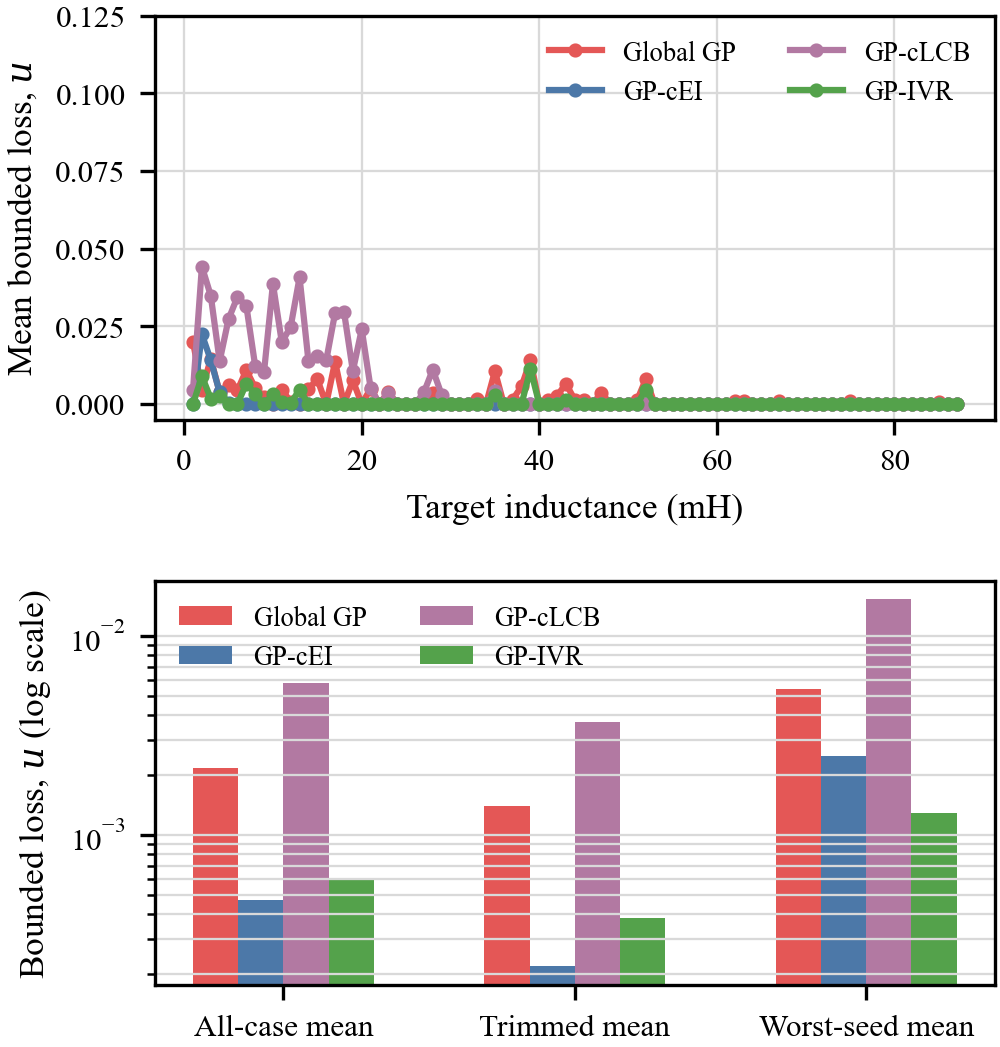
\includegraphics[width=0.98\columnwidth]{fig04_gp_acquisition_comparison.png}
 \caption{Matched target-conditioned acquisition comparison at $B=27$ over ten seeds and 87 targets. Lower bounded loss is better.}
 \label{fig:acquisition}
\end{figure}

\begin{figure*}[!t]
 \centering
 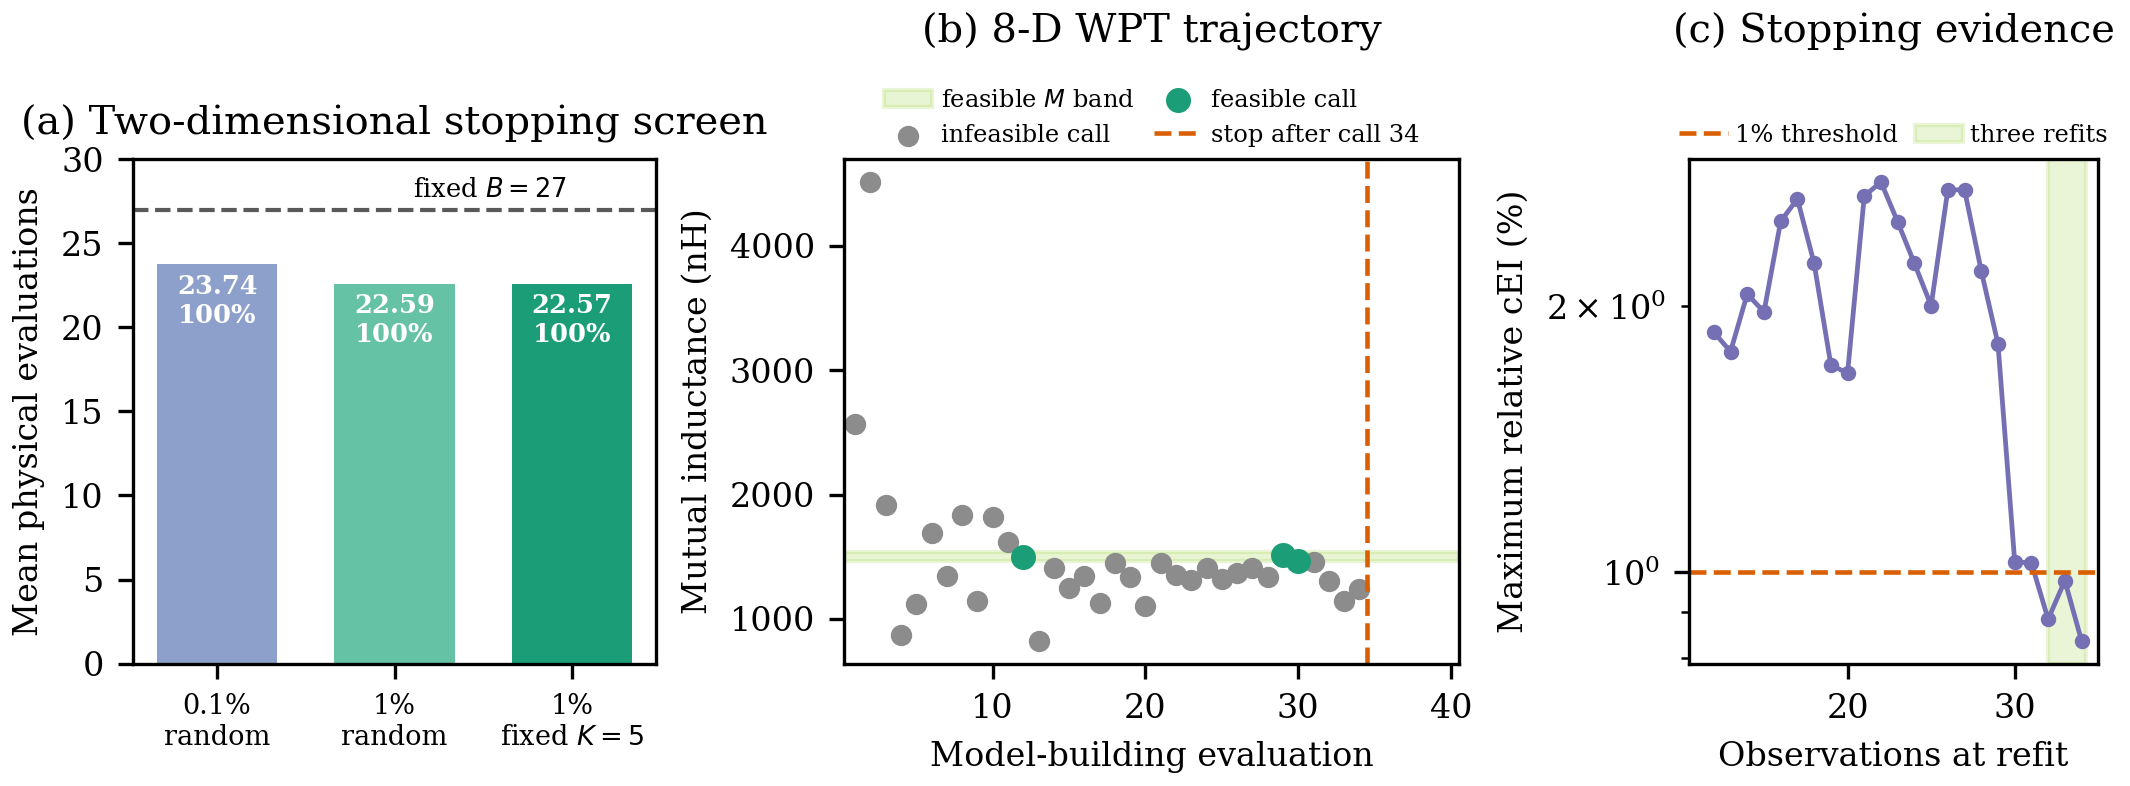
\includegraphics[width=0.90\textwidth]{fig05_automated_stopping.png}
 \caption{Automatic budgeting. (a) Mean total calls on the 14-target development screen; every configuration reaches the exhaustive optimum. (b) Model-building trace for the representative 1500-nH WPT transfer. (c) Maximum relative cEI after feasibility; three consecutive values below 1\% trigger stopping, followed by ten charged confirmations.}
 \label{fig:stopping}
\end{figure*}

\section{Eight-Dimensional WPT Transfer}
\subsection{Controlled Black-Box Benchmark}
The source WPT model has eight intrinsic geometry variables and six pose variables \cite{asadi2025}. We optimize the eight geometry variables: polygon side count $n_s\in[4,10]$, turn count $n_t\in[5,15]$, spacing $s\in[1,3]$ mm, and inner radius $r_i\in[30,80]$ mm for each transmitter and receiver. The counts are integral; $s$ and $r_i$ are continuous. Translation is fixed at $(0,0,70)$ mm and rotations are zero, so the task makes no tolerance or misalignment claim.

The constraint is $|M(x)-M_t|/M_t\leq0.025$. Total DC resistance is computed from polygonal conductor centerline length,
\begin{equation}
 R=\frac{\rho_{\rm Cu}}{A}\sum_{q\in\{t,r\}}\sum_{k=0}^{n_{t,q}-1}
 2n_{s,q}r_{q,k}\sin(\pi/n_{s,q}),
 \label{eq:wpt-r}
\end{equation}
where $r_{q,k}=r_{i,q}+k(s_q+w)$, $w=0.68$ mm, $A=\pi(w/2)^2$, and $\rho_{\rm Cu}=1.851\times10^{-5}\ \Omega\,\mathrm{mm}$. Leads are excluded. The partial-inductance oracle follows \cite{asadi2025}.

This numerical model is a controlled black-box benchmark: both responses are hidden and learned by separate GPs. It measures observation efficiency under equal oracle-call accounting, while the direct Maxwell experiment below tests field-solver execution rather than wall-clock acceleration.

The normalized center is evaluated first. Consecutive blocks of one unscrambled Sobol sequence provide deterministic candidates. Isotropic Mat\'ern-$5/2$ GPs use the same fixed $K=5$ fitting, 75/25 feasibility rule, 1\% stopping threshold, patience three, and ten confirmations. With $d=8$, $N_{\min}=17$; at most 40 model-building calls plus ten confirmations are allowed. No setting is retuned after the 2-D study.

\subsection{Results}
Across the 21 targets, automatic and conventional cEI both qualify 21/21, versus 10/21 for Sobol. Their mean resistances are $0.31500$ and $0.31549\ \Omega$, but wins/ties/losses are 8/3/10, paired Wilcoxon $p=0.913$, and excluding 1250 nH reverses the ordering. Four trajectories end at the $2d+1=17$ guard. Thus the numerical evidence supports reliable feasibility and automatic budgeting, not resistance dominance.

\begin{table}[!t]
\caption{WPT transfer. $B_s$ and $R_s$ are the automatic stopping cost and resistance; $R_{50}$ is its forced-50 continuation. Five representative targets precede the full aggregate. Dashes are infeasible at the matched budget.}
\label{tab:wpt}
\centering
\scriptsize
\begin{tabular}{@{}rrrrrr@{}}
\toprule
$M_t$ (nH) & $B_s$ & $R_s$ & $R_{50}$ & Conv. & Sobol \\
\midrule
1000 & 33 & .2597 & .2597 & .2597 & -- \\
1250 & 34 & .2915 & .2803 & .3404 & -- \\
1500 & 44 & .3058 & .3058 & .3056 & .3439 \\
1750 & 27 & .3325 & .3249 & .3325 & -- \\
2000 & 27 & .3770 & .3437 & .3711 & .4228 \\
\midrule
Mean (21) & 34.86 & .31500 & .30350 & .31549 & -- \\
Qualified & -- & 21/21 & 21/21 & 21/21 & 10/21 \\
\bottomrule
\end{tabular}
\end{table}

Twenty runs stop naturally; 1150 nH reaches the 40-call cap. Versus forced $B=50$, stopping uses 30.3\% fewer observations for 3.79\% higher mean resistance, so a 1\% posterior threshold is not a 1\% realized-gap guarantee. At 1500 nH, $M=1466.48$ nH and $R=0.30577\ \Omega$; the 3.98-nH lower-bound margin implies nominal, not manufacturing-robust, feasibility.

\subsection{Field-Solver Application Check}
At 1000 nH, the frozen automatic workflow stops naturally after 20 model-building calls and then performs ten frozen confirmations. A matched baseline uses six fixed Sobol points, 14 conventional-cEI calls, and ten confirmations. Both qualify, but the automatic run yields seven feasible observations, $M=998.929$ nH, and $R_{\rm AC,Tx}+R_{\rm AC,Rx}=0.383681\ \Omega$; the baseline yields three, $1016.402$ nH, and $0.389535\ \Omega$. Thus the automatic objective is 1.50\% lower despite the baseline's deterministic Sobol initialization. This is one trajectory per policy, not statistical dominance: the baseline finds feasibility earlier (call 6 versus 12), and the two winners require a common mesh-convergence check before the small objective gap is treated as definitive.

In the numerical 1500-nH example, Tx/Rx use 9/7 sides, 7/7 turns, 1.741/2.709-mm spacing, and 61.724/61.007-mm inner radii. Feasibility occurs at model call 12; stopping at 34 plus ten confirmations gives $B=44$, and forced continuation returns the same design. The 21-target aggregate, not this example, supports numerical transfer.

\begin{figure}[!t]
 \centering
 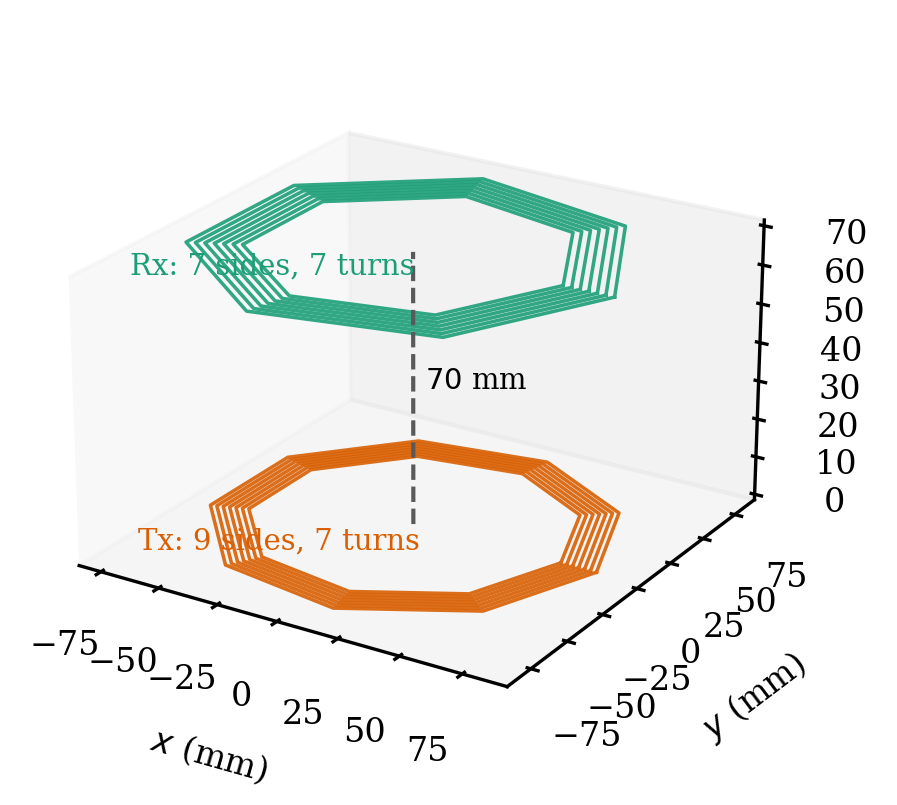
\includegraphics[width=0.82\columnwidth]{fig06_wpt_selected_geometry.png}
 \caption{Selected nominal-pose 1500-nH design. The aligned transmitter and receiver planes are separated by 70 mm; the illustration does not represent a misalignment study.}
 \label{fig:wpt-geometry}
\end{figure}

\section{Discussion and Conclusion}
The experiments support a compact engineering policy: begin from a declared center, mix predicted feasibility with constraint uncertainty only until a feasible observation exists, fit each GP from fixed low-discrepancy hyperparameter starts, require at least $2d+1$ observations, and stop only after persistent low relative cEI while charging terminal checks explicitly. This removes implementation-level seed variation and performs consistently across the complete 2-D target lattice. Its transfer advantage is reliable feasibility and adaptive cost, not universally lower resistance.

The conclusions remain bounded. The 2-D oracle is analytical, the 21-target WPT screen uses one nominal pose and a partial-inductance model, and Maxwell contributes one trajectory per policy. This demonstrates field-solver transfer, not experimental validation or general superiority; the winners still need common mesh convergence. The 75/25 weight and stopping rule are empirical, and noise, sparse candidates, discontinuity, or kernel misspecification can invalidate them. Code and complete evidence are public at \url{https://github.com/baolinhnguyen013a-dotcom/reproducible-target-informed-gp}.

\begin{thebibliography}{00}
\bibitem{rasmussen} C. E. Rasmussen and C. K. I. Williams, \emph{Gaussian Processes for Machine Learning}. MIT Press, 2006.
\bibitem{gardner} J. Gardner, M. Kusner, Z. Xu, K. Weinberger, and J. Cunningham, ``Bayesian optimization with inequality constraints,'' in \emph{Proc. ICML}, vol. 32, 2014, pp. 937--945.
\bibitem{liu2014} B. Liu \emph{et al.}, ``An efficient method for antenna design optimization based on evolutionary computation and machine learning techniques,'' \emph{IEEE Trans. Antennas Propag.}, vol. 62, no. 1, pp. 7--18, 2014.
\bibitem{wu2024} Q. Wu, W. Chen, C. Yu, H. Wang, and W. Hong, ``Machine-learning-assisted optimization for antenna geometry design,'' \emph{IEEE Trans. Antennas Propag.}, vol. 72, no. 3, pp. 2083--2095, 2024.
\bibitem{sim2023} B. Sim \emph{et al.}, ``Bayesian optimization based fast and accurate wireless power transfer system coil optimization for high efficiency,'' in \emph{Proc. IEEE WPTCE}, 2023.
\bibitem{asadi2025} M. Asadi and A. M. Abazari, ``A data-driven model to predict mutual inductance between planar coils with arbitrary specifications and positions,'' \emph{IET Electr. Power Appl.}, vol. 19, Art. no. e70015, 2025.
\bibitem{furuuchi2024} S. Furuuchi and S. Yamada, ``Verifying the effect of initial sample size in Bayesian optimization,'' \emph{Total Quality Science}, vol. 10, no. 1, pp. 8--19, 2024.
\bibitem{ishibashi2023} H. Ishibashi, M. Karasuyama, I. Takeuchi, and H. Hino, ``A stopping criterion for Bayesian optimization by the gap of expected minimum simple regrets,'' in \emph{Proc. AISTATS}, vol. 206, 2023, pp. 6463--6497.
\bibitem{kirkpatrick} S. Kirkpatrick, C. D. Gelatt, Jr., and M. P. Vecchi, ``Optimization by simulated annealing,'' \emph{Science}, vol. 220, no. 4598, pp. 671--680, 1983.
\end{thebibliography}

\end{document}
